Similmente al comportamento stellare anche le galassie possono raggrupparsi in \emph{gruppi} o \emph{ammassi}.
Un gruppo di galassie è solitamente caratterizzato da un numero di elementi che si aggira intorno alla decina, mentre un ammasso è una struttura che può contare dalle $100$ alle $1000$ galassie tenute insieme dall’interazione gravitazionale.

\section{Gruppi di galassie}\label{sec:gruppi-di-galassie}
Nonostante sia impossibile determinare in maniera precisa ed univoca le caratteristiche dei gruppi di galassie, si cerca di esporre le più comuni. 
I gruppi di galassie presentano un numero di elementi minore a $50$ e un’estensione radiale $R \leq 0.5$--$\SI{1}{Mpc}$. Alcuni gruppi sono particolarmente compatti ($R \sim \SI{100}{kpc}$) e vengono chiamati \emph{gruppi di Hickson}. 
Le galassie che formano il gruppo sono solitamente galassie a disco o di forma irregolare e la massa totale del gruppo è dell’ordine delle $10^{13}$ masse solari. 
Per un gruppo, la dispersione di velocità è di circa $\sigma \sim 100$--$\SI{500}{km.s^{-1}}$ : queste velocità sono considerabili lente e fanno sì che la probabilità di interazione fra le galassie sia maggiore rispetto al caso degli ammassi (cap.~\ref{sec:ammassi-di-galassie}) contribuendo così alla formazione di una morfologia irregolare.
I gruppi emettono radiazione elettromagnetica in banda X tramite processi legati al gas caldo diffuso che li permea (si veda par.~\ref{sec:intra-cluster-medium}).
Infine il rapporto massa-luce M/L, ovvero il parametro dato dal quoziente tra la massa totale e la luminosità del gruppo, varia nel range $100$--$300$.

\noindent Si noti come quest’ultimo parametro sia in grado di fornire informazioni sulla quantità di materia oscura presente: essa, infatti, contribuisce alla massa complessiva, ma non alla radiazione elettromagnetica emessa. 
\subsection{Il Gruppo Locale}
La nostra galassia, la Via Lattea, fa parte di un gruppo galattico detto Gruppo Locale (figura~\ref{fig:gruppo-locale}) che conta un numero di $70$/$80$ galassie. Due di esse sono particolarmente importanti in quanto le più grandi e luminose: la Via Lattea e la galassia di Andromeda, chiamata anche M31.
La massa totale del gruppo è di “sole” $10^{12}$ masse solari e ha un’estensione radiale di $\SI{1.5}{Mpc}$.
Presenta una moltitudine di stelle risolte nel diagramma di magnitudine CMD.

\noindent Il gruppo è suddivisibile in due sottogruppi, uno legato alla Via Lattea e l’altro ad M31, i quali si stanno avvicinando con una velocità relativa di circa $\SI{120}{km.s^{-1}}$.
Le dimensioni e la morfologia delle galassie appartenenti al Gruppo Locale è vasta, sono infatti presenti: nane sferoidali, nane ellittiche, nane irregolari e galassie a spirale. Solo tre galassie hanno quest’ultima struttura: Andromeda, la Via Lattea e M33 (denominata Galassia del Triangolo).
Inoltre il Gruppo Locale fa parte di un raggruppamento più grande, il \emph{Superammasso della Vergine}, rappresentato in figura \ref{fig:virgo-cluster} e composto da più di $100$ sotto gruppi e ammassi di galassie. Il nome deriva dall’ammasso della Vergine, l'ammasso più grande che gli appartiene (con una massa di $10^{15}$ masse solari!).
\begin{figure}
    \centering
    \includegraphics[width = 0.5\textwidth]{immagini/Gruppo-Locale.png}
    \caption{Schema del Gruppo Locale}
    \label{fig:gruppo-locale}
\end{figure}
\begin{figure}
    \centering
    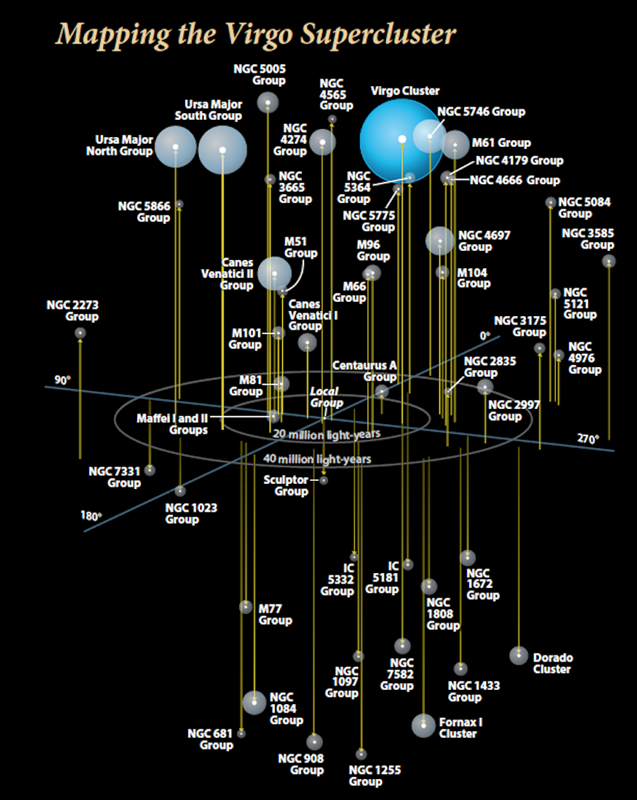
\includegraphics[width = 0.5\textwidth]{immagini/virgo-cluster.png}
    \caption{Rappresentazione del \emph{super ammasso} della Vergine, la sfera azzurra è l'\emph{ammasso} della Vergine da cui prende il nome}
    \label{fig:virgo-cluster}
\end{figure}
\subsection{Ultra-faint galaxies}
Recenti osservazioni hanno trovato un elevato numero di \emph{ultra-faint spheroidal dwarfs} (letteralmente galassie nane sferoidali molto deboli) che sono caratterizzate da luminosità molto basse ($M \sim {-1.5}$), dimensioni paragonabili ad ammassi globulari (decine di Parsec) e metallicità bassissime che indicano la presenza di materiale primordiale non arricchito da precedenti popolazioni. La caratteristica più degna di nota è l’altissimo rateo massa-luce ($\geq 1000$): pochissima luce, ma un’elevatissima massa.
Queste galassie sono delle ottime candidate per futuri studi sulla materia oscura.
